\section{Introduction}
\label{sec:intro}

\begin{figure}[htbp]
\centering
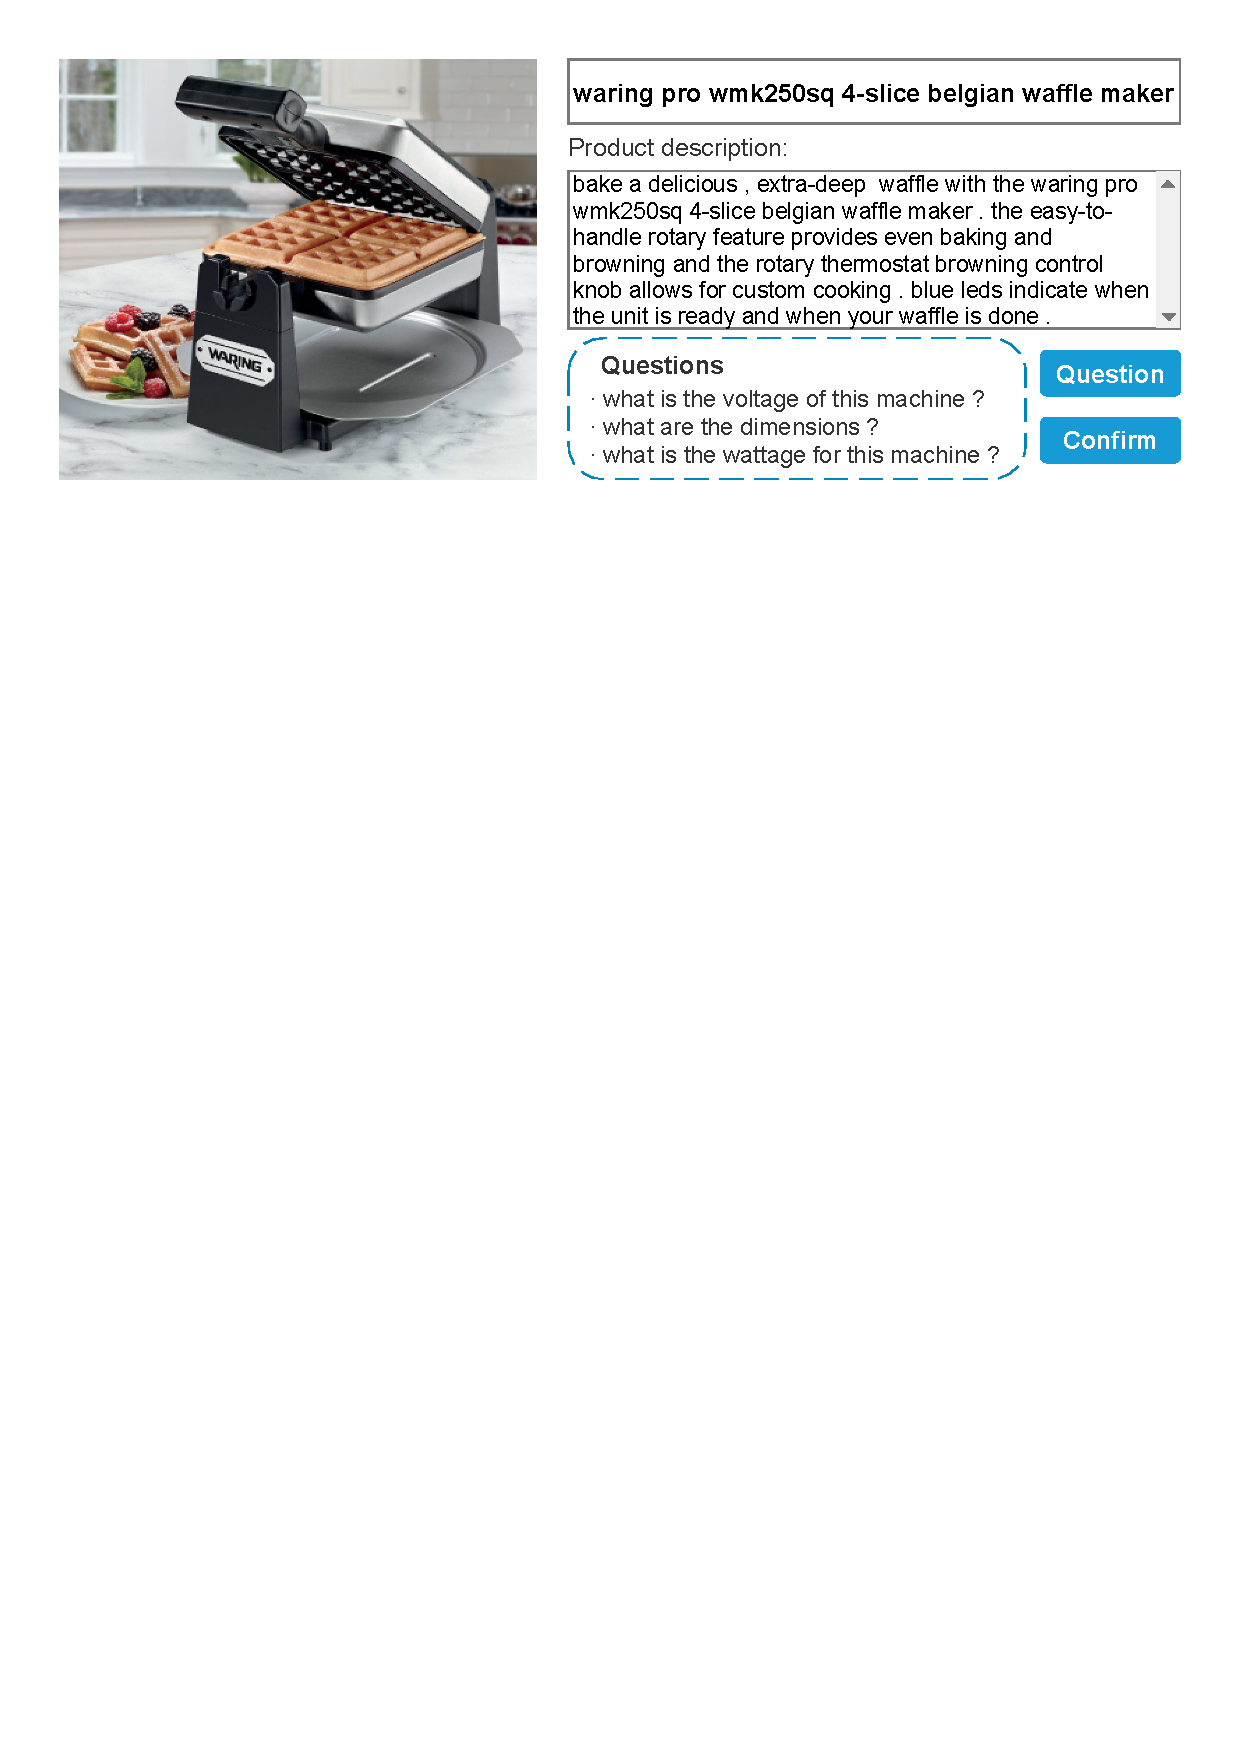
\includegraphics[width=\linewidth]{WA_UI.pdf}
\caption{A hypothetical writing assistant generating CQs.}
\label{fig:WA_UI}
\end{figure}
  
The development of the Internet has spawned a number of task-oriented writings, such as product descriptions on Amazon. However, since merchants cannot always have a thorough understanding of consumers' need due to the variety of possible user backgrounds and use cases, their writings usually miss something deemed important by the customers. For example, a US merchant may assume his device be 
used on a 110V power line, and thus omit this in the product description. 
Customers from Asia and Europe, where 220V is used, might pay special attention to the voltage 
requirements in the description. On finding this absent from the description, 
some customers may ask CQs like ``What is the voltage of this machine?'' in customer QA, while others would turn to other products immediately, an unfortunate loss to the seller. It would be helpful if the platform can provide a service to remind the merchants of those potentially missing needs with its broader knowledge.


Clarification question\footnote{questions asking for what's missing from a given context} generation (CQGen), which mimics the user engagement by raising questions, can be a promising option for such a service. Before publishing their writings, authors may request for CQs from somewhere like the hypothetical writing assistant we illustrated in Figure \ref{fig:WA_UI}, and supplement missing information accordingly. CQGen is a challenging task for the following reasons: 

First, it requires the question to be 
\textit{specific} while not being \textit{repetitive} to existing context. 
Questions pertaining to smaller set of products are considered more specific. 
For example, the first question in Figure \ref{fig:WA_UI} is more specific 
than the second one because it applies to only electric appliances, while
the second one applies almost to every product. 
In contrast to the traditional QGen task which is typically evaluated
on the SQuAD 1.1 dataset \citep{rajpurkar2016squad} and 
derives the specificity from the knowledge of answer, 
CQGen doesn't expect the existence of answer in the context. 
Therefore, QGen algorithms which require the answer span and its position
as input~\citep{song2018leveraging, sun2018answer,subramanian2018neural} 
do not apply here. Vanilla seq2seq model has been shown to generate 
highly generic questions by \citet{rao2019answer}. 
They then proposed GAN-Utility, which estimates the utility of answer with GAN 
as reward for RL to improve generation specificity. 
However, the answer used in the estimation is generated from the context and an already-generated 
question with another trained QA component, 
which may not be reliable here as the answers are inherently 
missing from context by definition. 
Consequently, this answer-based approach was shown to yield even worse results under 
some conditions~\citep{cao2019controlling}. We thus totally eliminate the need for answers in our work, 
which has the benefit of making use of more training data without answer.

Moreover, previous works on CQGen all assume generating one question per context. We claim that generating a group of diverse CQs 
(as is shown in Figure \ref{fig:WA_UI}) can be more beneficial, 
because this allows the system to efficiently cover a variety of user 
needs at once, and tolerate occasional errors as the rest questions are still useful. 
We name this novel task as \textbf{Diverse CQGen}. We seek algorithms that can deal with the task, and adopt a new group-level evaluation protocol to properly evaluate the effectiveness of algorithms under this scenario.

To deal with the specificity challenge, we propose a novel model named 
Keyword Prediction and Conditioning Network (KPCNet). Keywords in CQs is one kind of prior knowledge that the platform can mine about user needs. They are usually
product attributes or closely related concepts that make the questions specific, and thus the main semantic of a question can be captured by its keywords. 
For example, the keyword of ``What's the \textit{dimension}?'' 
is ``\textit{dimension}'', and the question can be comprehended even with 
a single word (``\textit{dimension}?''). We can generate more detailed question like ``Can you cook \textit{rice} in this \textit{cooker}?'' with keywords ``\textit{cooker, rice}''. 
Therefore, the proposed KPCNet first predicts 
the probability for a keyword to appear in the generated CQ, 
then selects keywords from the predicted distribution, 
and finally conditions on them to generate questions. 
We can also partially control the generation by operating on the 
conditioned keywords, which can be utilized to avoid repetitive questions 
and further improve the quality.

To promote diversity, we explore several diverse generation approaches for 
this problem, including model-based 
\textit{Mixture of Experts}~\citep{shen2019mixture} and 
decoding-based \textit{Diverse Beam Search} \citep{vijayakumar2018diverse}. 

KPCNet's controllability through keywords, on the other hand, 
enables keywords-based approaches. We explore a novel use of classic
clustering method on producing coherent keyword groups for keyword selection 
to generate correct, specific and diverse questions.

Individual and group-level evaluation showed that KPCNet is capable of 
producing more diverse and specific questions than strong baselines. 
Our contributions are:

\begin{enumerate}
  \item To our best knowledge, we are the first to propose the 
task of \textit{Diverse CQGen}, which requires generating a group of 
diverse CQs per context, to cover a wide range of information needs.  
(\S \ref{sec:intro})
  \item We propose KPCNet, which first predicts keywords that focus on the specific aspects of the question, 
before generating the whole question to promote specificity. (\S \ref{sec:specific}, \S \ref{sec:prediction})

  \item Based on KPCNet's keyword conditioned generation, we propose keyword selection methods to produce multiple keywords groups for generation diversity. (\S \ref{sec:diversity}, \S \ref{sec:cond_gen}, \S \ref{sec:selection})
  \item We show with probing tests that KPCNet can be further enhanced with external knowledge to alleviate the problem of asking existing information in the context, an under-explored yet fundamental problem in CQGen, and improve generation quality. (\S \ref{sec:probing})
\end{enumerate}

